% This file was created by matlab2tikz.
%
%The latest updates can be retrieved from
%  http://www.mathworks.com/matlabcentral/fileexchange/22022-matlab2tikz-matlab2tikz
%where you can also make suggestions and rate matlab2tikz.
%
\definecolor{mycolor1}{rgb}{0.00000,0.44700,0.74100}%
\definecolor{mycolor2}{rgb}{0.85000,0.32500,0.09800}%
%
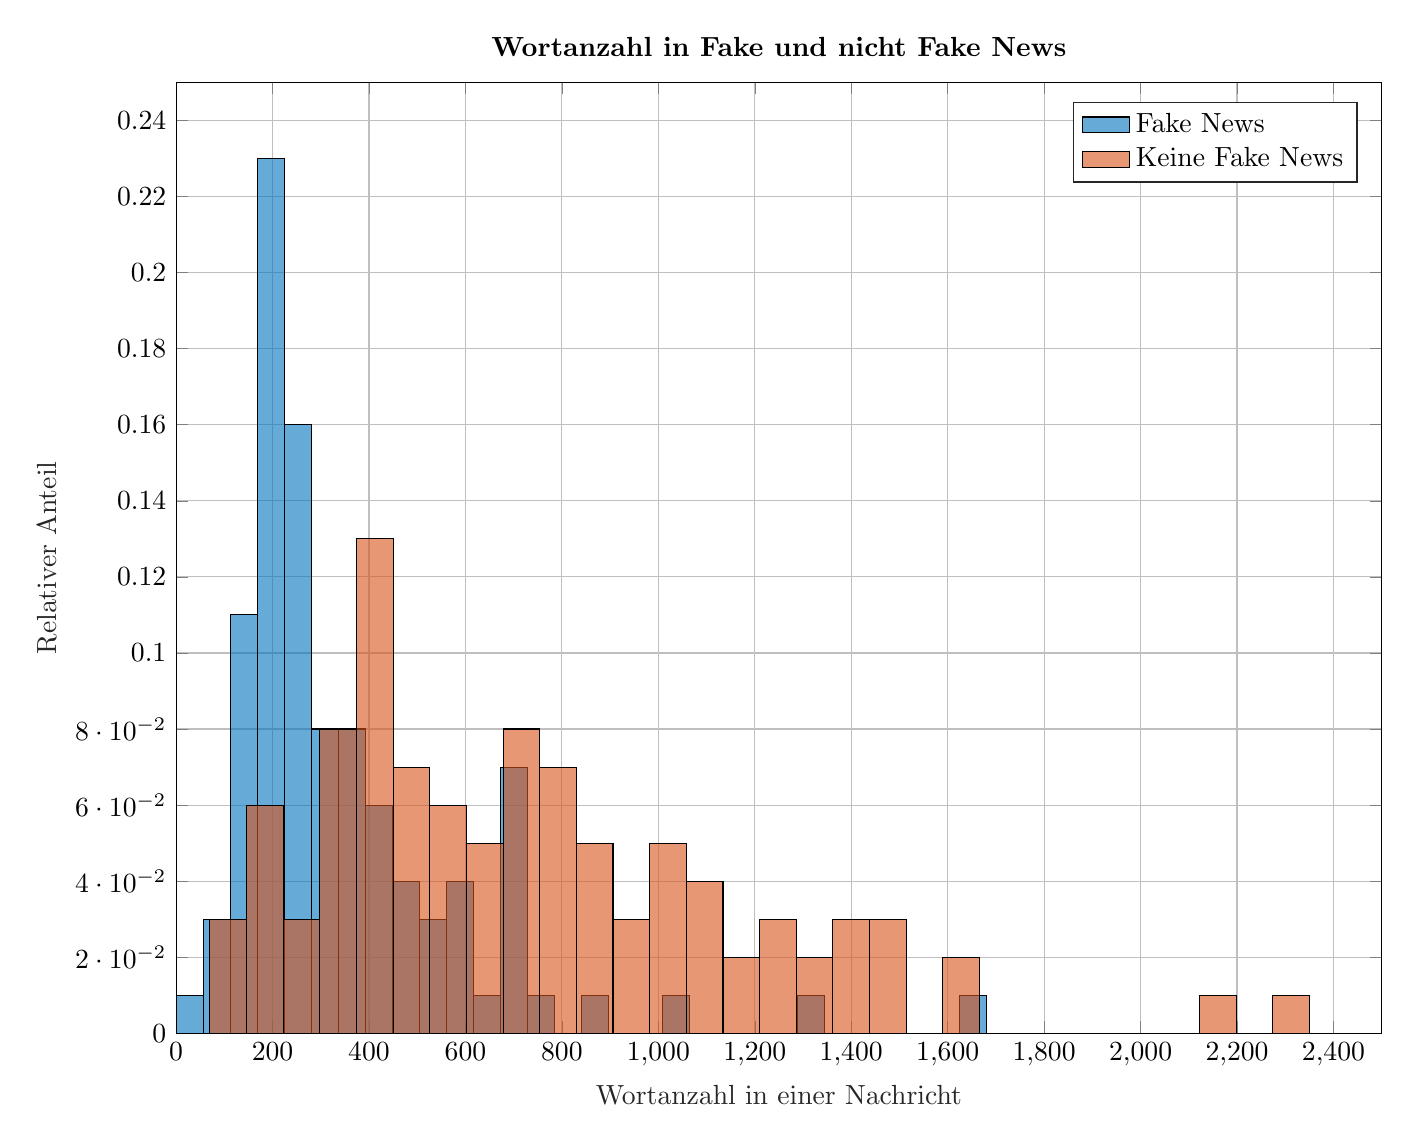
\begin{tikzpicture}

\begin{axis}[%
width=6.028in,
height=4.754in,
at={(1.011in,0.642in)},
scale only axis,
xmin=0,
xmax=2500,
xlabel style={font=\color{white!15!black}},
xlabel={Wortanzahl in einer Nachricht},
ymin=0,
ymax=0.25,
ylabel style={font=\color{white!15!black}},
ylabel={Relativer Anteil},
axis background/.style={fill=white},
title style={font=\bfseries},
title={Wortanzahl in Fake und nicht Fake News},
xmajorgrids,
ymajorgrids,
legend style={legend cell align=left, align=left, draw=white!15!black}
]
\addplot[ybar interval, fill=mycolor1, fill opacity=0.6, draw=black, area legend] table[row sep=crcr] {%
x	y\\
0	0.01\\
56	0.03\\
112	0.11\\
168	0.23\\
224	0.16\\
280	0.08\\
336	0.08\\
392	0.06\\
448	0.04\\
504	0.03\\
560	0.04\\
616	0.01\\
672	0.07\\
728	0.01\\
784	0\\
840	0.01\\
896	0\\
952	0\\
1008	0.01\\
1064	0\\
1120	0\\
1176	0\\
1232	0\\
1288	0.01\\
1344	0\\
1400	0\\
1456	0\\
1512	0\\
1568	0\\
1624	0.01\\
1680	0.01\\
};
\addlegendentry{Fake News}

\addplot[ybar interval, fill=mycolor2, fill opacity=0.6, draw=black, area legend] table[row sep=crcr] {%
x	y\\
70	0.03\\
146	0.06\\
222	0.03\\
298	0.08\\
374	0.13\\
450	0.07\\
526	0.06\\
602	0.05\\
678	0.08\\
754	0.07\\
830	0.05\\
906	0.03\\
982	0.05\\
1058	0.04\\
1134	0.02\\
1210	0.03\\
1286	0.02\\
1362	0.03\\
1438	0.03\\
1514	0\\
1590	0.02\\
1666	0\\
1742	0\\
1818	0\\
1894	0\\
1970	0\\
2046	0\\
2122	0.01\\
2198	0\\
2274	0.01\\
2350	0.01\\
};
\addlegendentry{Keine Fake News}

\end{axis}
\end{tikzpicture}%